\documentclass[11pt,a4paper]{article}

\usepackage[margin=1in]{geometry}
\usepackage{amsmath}
\usepackage{microtype}
\usepackage{hyperref}
\usepackage{enumitem}
\usepackage{graphicx}
\usepackage{xcolor}
\usepackage{array}
\usepackage{tikz}
\usepackage{float}

\usetikzlibrary{positioning}

\setlist[itemize]{leftmargin=0.7cm}
\setlist[enumerate]{leftmargin=0.7cm}
\setlength{\emergencystretch}{3em}

% -----------------------------------------------------
% bvraghav-tiet-ucs503p-article.sty
% -----------------------------------------------------

\makeatletter
\newcommand{\BvrSetLabInstructor}[1]{%
  \gdef\Bvr@LabInstructor{#1}}
\newcommand{\Bvr@LabInstructor}{}
\newcommand{\BvrLabInstructorValue}{\Bvr@LabInstructor}
\makeatother

\usepackage{titling}

\pretitle{\begin{center}\bfseries\fontsize{17.28pt}{21pt}\selectfont}

\makeatletter
\newcommand{\BvrSubtitle}[1]{%
  \posttitle{%
    \par\end{center}
    \begin{center}\large#1\end{center}
    \vskip 0.5em}%
}
\makeatother

\newcommand{\BvrHint}[1]{%
  \ifx&#1&%
  \else
    {\normalfont\normalsize\itshape\hfill #1}%
  \fi}

% -----------------------------------------------------

\title{CampusCare: An Integrated Digital Healthcare Platform for Campus Health Centers}

\BvrSetLabInstructor{}

\BvrSubtitle{%
  Project Proposal for UCS503P \\
  Submitted to: Ms. Anushka\BvrLabInstructorValue \\
  \textbf{Thapar Institute of Engineering and Technology}%
}

\author{%
  Lavdeep Singh, CSED%
  \thanks{Roll No: \texttt{1024030107},%
    Email: \texttt{lsingh2\_be24@thapar.edu}}%
  \and
  Harshveer Singh, CSED%
  \thanks{Roll No: \texttt{1024030109},%
    Email: \texttt{hsingh\_be24\@thapar.edu}}%
  \and
  Damanbir Singh, CSED%
  \thanks{Roll No: \texttt{1024030110},%
    Email: \texttt{dsingh5\_be24\@thapar.edu}}%
  \and
  Kriti, CSED%
  \thanks{Roll No: \texttt{1024030111},%
    Email: \texttt{kkriti\_be24\@thapar.edu}}%
}

\date{August 19, 2026}

\begin{document}

\maketitle

% =====================================================
% 1. HIGHER-ORDER GOAL
% =====================================================

\section{Higher order goal \BvrHint{}}

The campus health center currently runs on manual processes, and this creates real friction for students and staff alike. Our goal is to reduce that time: shorter waits, easier access to medical history, and a consultation to dispensation process that doesn't depend on paper.

That's the broader aim. The concrete engineering goal, the one we can actually plan and build toward, is turning the health center's existing manual workflow into a system we can measure and deploy.

The system we're proposing ties together student identity, health records, doctor specific queues, consultation notes, structured prescriptions, medicine dispensing, and administrative controls, all under one role-based platform.

We're deliberately staying out of clinical decision making. Students and staff will still choose which doctor to see, and emergency cases will run through their own workflow instead of sitting in the regular queue.

% =====================================================
% 2. TIME-TO-VALUE
% =====================================================

\section{Time to value \BvrHint{}}

\begin{itemize}
    \item We're building the smallest complete version of the healthcare workflow first: check in, doctor queue, consultation, prescription, dispensing, and visit completion. That gives us something real to test early instead of a pile of half finished features.
    \item A working end to end flow comes before trying to build every planned feature at once.
    \item Check in will start out staff assisted and manual, so we can validate the core workflow before we touch NFC or RFID integration at all.
    \item NFC/RFID support only gets added once we've actually tested whether the college ID card, the target Android device, the browser, and our deployment setup all work together.
    \item We will work in short iterations with continuous testing, so problems in the core workflow surface early rather than after we've built more on top of them.
    \item CI/CD gets set up early so every change is automatically built, tested, and pushed to a staging environment.
    \item In the first iteration, success means a full healthcare visit can be processed correctly, not how many features got built.
\end{itemize}

% =====================================================
% 3. PROBLEM STATEMENT
% =====================================================

\section{Problem Statement}

Right now, the campus health center leans heavily on manual processes for check in, queue management, consultation records, prescriptions, and dispensing. That creates a handful of recurring problems:

\begin{itemize}
    \item \textbf{Unclear queue status:} students often wait without knowing where they stand in line or how many people are ahead of them.
    \item \textbf{Limited access to medical history:} doctors don't always have quick access to a student's past visits, prescriptions, or relevant conditions, so consultations can start without that context.
    \item \textbf{Paper based prescriptions:} handwriting is hard to read, papers get lost, and there's no structured digital record to fall back on during a future visit.
    \item \textbf{Weak dispensing records:} what a doctor prescribes and what a student actually receives aren't always tied together in one system.
    \item \textbf{Manual identity checks:} students without their ID card need staff to verify and check them in by hand.
    \item \textbf{Scattered information:} identity, health profile, visit history, prescriptions, queue state, and dispensing details often live across separate, disconnected processes.
    \item \textbf{Limited administrative oversight:} doctor availability, staff accounts, and card enrollment all need a central place to be managed.
    \item \textbf{Routine and emergency cases don't mix well:} the two need different handling, and forcing them through the same queue doesn't work.
\end{itemize}

\textbf{Why this matters now:} the health center deals with a steady stream of students but has limited medical and administrative staff. Making the queue more transparent, records easier to reach, and the workflow better coordinated can cut down on avoidable waiting and repeated paperwork, while making care more continuous for students.

% =====================================================
% 4. PROPOSED SOLUTION
% =====================================================

\section{Proposed Solution \BvrHint{}}

\subsection{Overview}

We're building a \textbf{web based Progressive Web App (PWA)} that digitizes the routine campus healthcare workflow, with clear roles for students, doctors, pharmacists/receptionists, and administrators.

The system will include:

\begin{itemize}
    \item \textbf{Student portal:} students set up and maintain their profile, add relevant medical information, view their history and prescriptions, check in, pick an available doctor, and track their queue status.
    \item \textbf{Identity assisted check in:} we'll look into using the existing college ID card as an NFC/RFID check in method, linking its identifier to the student's account. Staff assisted manual check in stays available whenever the card isn't an option.
    \item \textbf{Doctor specific queues:} students join the queue of the doctor they've chosen and can see where they stand.
    \item \textbf{Doctor consultation workflow:} doctors call students in, pull up relevant history, log the consultation, write structured prescriptions, and redirect a student to another doctor's queue when needed.
    \item \textbf{Structured prescriptions:} prescriptions use dedicated fields for medication and dosage, plus a general instructions section, instead of relying purely on free form text.
    \item \textbf{Pharmacist/receptionist workflow:} handles manual check ins, verifies and logs what medicine was actually dispensed, and closes out completed visits.
    \item \textbf{Emergency recording:} emergency and trauma cases go through a separate workflow run by designated emergency staff, rather than joining the routine queue.
    \item \textbf{Administrative dashboard:} admins manage doctor and pharmacist/receptionist accounts, doctor availability, student related admin info, and card enrollment.
    \item \textbf{Role based access control:} what a user can see and do depends on their assigned role.
    \item \textbf{Audit logging:} important actions get recorded along with who did them and when, for accountability.
\end{itemize}

\subsection{Core workflow}

\begin{enumerate}
    \item A student logs into CampusCare using their own profile.
    \item At the health center, the student checks in with their college ID card if NFC/RFID support is live and working. If not, the pharmacist/receptionist checks them in manually.
    \item The student picks an available doctor and joins that doctor's queue.
    \item The student can check their queue status any time from their CampusCare account.
    \item The doctor calls the next student when ready.
    \item The doctor pulls up the student's health profile and past clinical records.
    \item The doctor logs the consultation and writes a structured prescription.
    \item If a student ends up with the wrong doctor, that doctor can redirect the visit to the right queue without creating a duplicate.
    \item After the consultation, the visit moves into a dispensing state.
    \item The pharmacist/receptionist verifies and logs the medicines actually dispensed.
    \item The doctor's original prescription stays untouched as the clinical record. Any difference between what was prescribed and what was dispensed gets recorded separately, not overwritten.
    \item Once dispensing is done, the visit closes and becomes part of the student's medical history.
    \item Emergency and trauma cases skip the routine queue entirely and go through the separate emergency workflow.
\end{enumerate}

\subsection{System Workflow}

The proposed system follows an end-to-end workflow beginning with physical identification and check-in, followed by visit creation, doctor-specific queue assignment, consultation, prescription, medicine dispensing, and permanent record storage.

\begin{figure}[H]
\centering

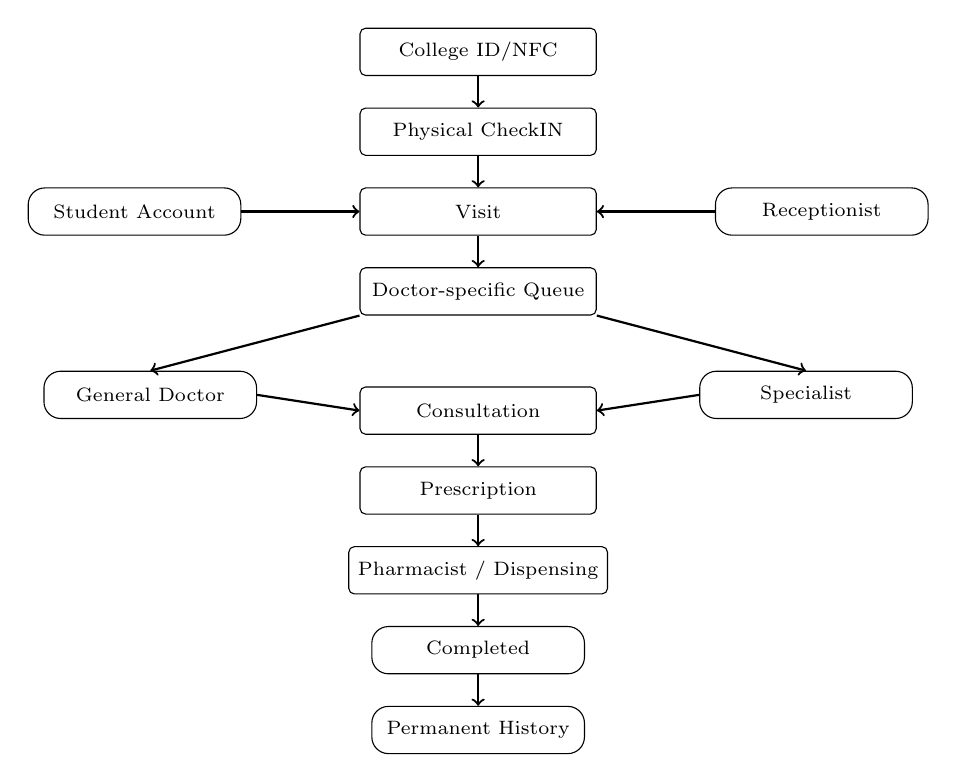
\begin{tikzpicture}[
    font=\scriptsize,
    process/.style={
        draw,
        rounded corners=2pt,
        minimum width=30mm,
        minimum height=6mm,
        align=center
    },
    actor/.style={
        draw,
        rounded corners=6pt,
        minimum width=27mm,
        minimum height=6mm,
        align=center
    },
    arrow/.style={
        ->,
        thick
    }
]

% MAIN FLOW
\node[process] (id) {College ID/NFC};
\node[process, below=4mm of id] (checkin) {Physical CheckIN};
\node[process, below=4mm of checkin] (visit) {Visit};
\node[process, below=4mm of visit] (queue) {Doctor-specific Queue};

% DOCTOR BRANCHES
\node[actor, below left=7mm and 13mm of queue] (general) {General Doctor};
\node[actor, below right=7mm and 13mm of queue] (specialist) {Specialist};

% CONSULTATION
\node[process, below=9mm of queue] (consultation) {Consultation};

% REMAINING FLOW
\node[process, below=4mm of consultation] (prescription) {Prescription};
\node[process, below=4mm of prescription] (pharmacy) {Pharmacist / Dispensing};
\node[actor, below=4mm of pharmacy] (completed) {Completed};
\node[actor, below=4mm of completed] (history) {Permanent History};

% SIDE ACTORS
\node[actor, left=15mm of visit] (student) {Student Account};
\node[actor, right=15mm of visit] (receptionist) {Receptionist};

% CONNECTIONS
\draw[arrow] (id) -- (checkin);
\draw[arrow] (checkin) -- (visit);
\draw[arrow] (visit) -- (queue);

\draw[arrow] (student.east) -- (visit.west);
\draw[arrow] (receptionist.west) -- (visit.east);

\draw[arrow] (queue.south west) -- (general.north);
\draw[arrow] (queue.south east) -- (specialist.north);

\draw[arrow] (general.east) -- (consultation.west);
\draw[arrow] (specialist.west) -- (consultation.east);

\draw[arrow] (consultation) -- (prescription);
\draw[arrow] (prescription) -- (pharmacy);
\draw[arrow] (pharmacy) -- (completed);
\draw[arrow] (completed) -- (history);

\end{tikzpicture}

\caption{End-to-end workflow from physical check-in to consultation, prescription, dispensing, and permanent history.}
\label{fig:healthcare_workflow}
\end{figure}

\subsection{Operational constraints for a campus setting}

\begin{itemize}
    \item The app needs to work well on the devices students and staff already have, so we're using responsive design and PWA features rather than assuming specific hardware.
    \item We're not trying to automate diagnosis or clinical decisions. The focus stays on workflow, access control, data integrity, and correctness.
    \item We'll rely on common cloud hosting and managed database services so the system doesn't need dedicated infrastructure to run.
    \item NFC/RFID check in is built as a replaceable piece, so manual staff assisted check in still works if the hardware or browser support falls short.
\end{itemize}

% =====================================================
% 5. SOLUTION APPROACH
% =====================================================

\section{Solution Approach \BvrHint{}}

This is an engineering course project, so we're focused on workflow, system correctness, database design, security, authorization, queue management, and deployability, not on inventing new clinical algorithms.

\subsection{Structured prescriptions and dispensing \BvrHint{}}

Prescriptions will use structured fields rather than one open text box for everything.

Depending on how we finalize the model, each medication entry may include:

\begin{itemize}
    \item Medication name
    \item Strength
    \item Dosage amount
    \item Dosage unit
    \item Form
    \item Route
    \item Frequency or schedule
    \item Duration
    \item Before/after food instructions where relevant
    \item As needed instructions where relevant
    \item Additional instructions
\end{itemize}

We'll settle on the exact structure after looking at established healthcare data models and figuring out which fields actually make sense for a campus health center.

The system keeps a clear line between what the doctor prescribed and what the pharmacist dispensed:

\[
\text{Doctor's Prescription}
\;\neq\;
\text{Pharmacist's Dispensing Record}
\]

That way the pharmacist can log what was actually handed out without ever quietly changing the doctor's original prescription.

We may draw on ideas from established healthcare interoperability standards like HL7 FHIR for the prescription structure, without trying to implement the full standard.

\subsection{Web architecture \BvrHint{}}

We're using a standard 3 tier architecture:

\begin{itemize}
    \item \textbf{Frontend:} React, Vite, and Tailwind CSS, with separate interfaces for students, doctors, pharmacists/receptionists, and admins.
    \item \textbf{Backend API:} Python and FastAPI, handling authentication, authorization, student profiles, health records, check in, queue management, consultations, prescriptions, dispensing, emergency records, RFID enrollment, and admin operations.
    \item \textbf{Database:} PostgreSQL, storing users, student profiles, health information, RFID credentials, visits, queue entries, consultations, prescriptions, dispensing records, emergency cases, and audit logs.
\end{itemize}

We're writing SQL by hand and managing schema changes through version controlled migration files, rather than leaning on an ORM as the main database layer.

Business rules and authorization checks live on the backend, not just in the frontend.

\subsection{Authentication and authorization}

CampusCare gives students persistent accounts and gives staff authenticated accounts of their own.

There are four main roles:

\begin{itemize}
    \item \textbf{Student}
    \item \textbf{Doctor}
    \item \textbf{Pharmacist/Receptionist}
    \item \textbf{Administrator}
\end{itemize}

Students can see their own medical information and visit history. Doctors, pharmacists/receptionists, and admins get access based on their responsibilities, following a permission matrix we'll finalize as we go.

We'll decide on the exact student authentication method, including whether to integrate with the college's Google identity system, once we've checked what's technically and institutionally feasible.

\subsection{NFC/RFID identity integration}

We're planning to use the existing college ID card as the physical identity mechanism for check in.

The intended flow looks like this:

\[
\text{College ID Card}
\;\rightarrow\;
\text{Card Identifier}
\;\rightarrow\;
\text{Student Account}
\;\rightarrow\;
\text{CampusCare Visit}
\]

The card identifier itself isn't treated as the student's medical identity, it's just a pointer to their account.

Before we treat this as a confirmed dependency, we'll actually test whether the college card works with a browser based Web NFC approach.

\subsection{Queue management}

Each doctor gets their own queue.

The queue system needs to support:

\begin{itemize}
    \item Students joining a doctor's queue
    \item Viewing queue status
    \item Doctors calling the next student
    \item No show handling
    \item Doctor redirection
    \item Queue completion
    \item Doctor availability
\end{itemize}

If a called student doesn't show up, we'll use a set buffer window. Once that window passes, the student gets moved to the end of the queue and the doctor moves on to the next person.

We'll decide on the exact no show duration after watching how the actual health center workflow plays out.

\subsection{CI/CD and faster delivery}

We're using CI/CD to:

\begin{itemize}
    \item Automatically build the frontend and validate the backend on every change.
    \item Run unit and integration tests.
    \item Handle linting and other automated checks.
    \item Produce repeatable deployment artifacts.
    \item Push successful builds to a staging environment.
    \item Catch integration issues between the four of us early, instead of finding them right before a demo.
\end{itemize}

% =====================================================
% 6. EVALUATION CRITERION
% =====================================================

\section{Evaluation Criterion \BvrHint{}}

We're measuring success with metrics tied directly to the core healthcare workflow.

\subsection{Key performance indicator}

\textbf{Time to check in to queue entry:} the time from when the student clicks check in to when their queue entry is successfully created.

Events in the system will record timestamps:

\[
\text{Check in Started}
\;\rightarrow\;
\text{Identity Verified}
\;\rightarrow\;
\text{Doctor Selected}
\;\rightarrow\;
\text{Queue Entry Created}
\]

We don't want to commit to a goal number upfront. Let's establish a baseline from the current manual process and see where we want to set our target.

\begin{itemize}
    \item \textbf{Metric:} timestamps are created automatically by the system.
    \item \textbf{Baseline:} manual workflow as it exists today.
    \item \textbf{Attribution:} timestamps are from CampusCare directly, not estimates.
\end{itemize}

\subsection{Secondary evaluation metrics}

\begin{itemize}
    \item \textbf{Queue transparency:} can students actually tell which doctor they're seeing, where they stand in the queue, and whether they've been called.
    \item \textbf{Waiting time:} time from joining the queue to being called.
    \item \textbf{Visit completion time:} time from check in all the way through consultation, dispensing, and closing the visit.
    \item \textbf{Record accessibility:} how long it takes, or how many steps it takes, for a doctor to pull up a student's relevant past records.
    \item \textbf{Prescription completeness:} what percentage of prescriptions include all the required structured fields.
    \item \textbf{Dispensing accuracy:} what percentage of visits correctly record prescribed versus dispensed medicine, including any documented differences.
    \item \textbf{Reliability:} how available and stable the system is during the pilot period.
    \item \textbf{Authorization correctness:} how well the system blocks actions outside a user's role.
\end{itemize}

\subsection{Pilot validation plan \BvrHint{}}

\begin{itemize}
    \item Use synthetic student and medical data for development, testing, and demos.
    \item Only use real student medical data if the institution explicitly signs off and our deployment meets the required privacy and security standards.
    \item Bring in a representative mix of student, doctor, pharmacist/receptionist, and admin test users.
    \item Walk through real workflows: check in, doctor selection, queue monitoring, consultation, prescription creation, dispensing, visit completion, doctor redirection, no show handling, emergency recording, and admin tasks.
    \item Compare the system's metrics against what we observe from the existing manual process.
\end{itemize}

% =====================================================
% 7. SCALABILITY
% =====================================================

\section{Scalability \BvrHint{}}

We want this to scale both in theory and in practice.

\begin{enumerate}
    \item \textbf{Scalable in theory:} the system should handle growth in students, visits, doctors, records, and concurrent sessions by:
    \begin{itemize}
        \item keeping the frontend and backend separate,
        \item paginating large result sets,
        \item indexing common database queries,
        \item keeping the relational data normalized,
        \item using transactions for queue and visit state changes,
        \item keeping the API stateless wherever practical.
    \end{itemize}
    \item \textbf{Deployable in practice:} the system should run on common web hosting and managed database infrastructure:
    \begin{itemize}
        \item a managed PostgreSQL database,
        \item a platform hosted frontend and backend,
        \item environment based configuration,
        \item a CI/CD pipeline for staging and production.
    \end{itemize}
\end{enumerate}

% =====================================================
% 8. ENGINE AVAILABILITY
% =====================================================

\section{Engine availability heuristic}

We already have an existing battle tested engine that we can use to build CampusCare as a web application:

\begin{enumerate}
    \item \textbf{React + Vite:} for frontend development.
    \item \textbf{Tailwind CSS:} for composable responsive interfaces.
    \item \textbf{FastAPI:} for our REST API and server logic.
    \item \textbf{PostgreSQL:} for our relational database.
    \item \textbf{Raw SQL alongside migration tooling:} for explicit schema development and versioning.
    \item \textbf{Web NFC:} for browser based NFC interactions. This is the approach we'll try to validate with the physical college ID card and Android phone.
    \item \textbf{Authentication infrastructure:} to handle authentication so students and staff have persistent accounts.
    \item \textbf{Testing tooling:} for unit tests and integration tests.
    \item \textbf{CI/CD tooling:} to automate checks and deploy our services.
    \item \textbf{Managed cloud hosting:} to deploy our frontend and API.
    \item \textbf{Managed PostgreSQL hosting:} to put a cloud hosted database into staging, testing, or production.
\end{enumerate}

Building off of existing tools means we can focus on workflow, correctness, security, database design, and measurement.

% =====================================================
% 9. PROJECT SCOPE AND DELIVERABLES
% =====================================================

\section{Project scope and deliverables \BvrHint{}}

\subsection{Initial deliverable \BvrHint{}}

The first iteration covers the smallest complete healthcare workflow:

\begin{itemize}
    \item Student account and authentication
    \item Student profile
    \item Staff assisted manual check in
    \item Doctor selection
    \item One doctor's queue
    \item Queue position and status
    \item Doctor authentication
    \item Doctor calls the next student
    \item Doctor views relevant student medical history
    \item Doctor records the consultation
    \item Doctor creates a structured prescription
    \item Pharmacist/receptionist views the prescription
    \item Pharmacist/receptionist records medicine dispensing
    \item Visit completion
    \item Completed visit shows up in student history
    \item PostgreSQL persistence
    \item Backend REST API
    \item Basic role based authorization
    \item CI build and backend tests
    \item Deployment to a staging environment
\end{itemize}

The point here is proving a complete healthcare visit can move through the system successfully, not cramming in as many screens or optional features as possible.

\subsection{Subsequent deliverables}

\begin{itemize}
    \item A second doctor with an independent queue.
    \item Doctor availability management.
    \item Doctor redirection between queues.
    \item No show handling and queue reordering.
    \item Full student medical history and prescription history.
    \item A better clinical history interface for doctors.
    \item A more complete set of role based permission rules.
    \item NFC/RFID check in.
    \item RFID enrollment and revocation.
    \item Card to student identifier mapping.
    \item Emergency and trauma recording.
    \item Administrative dashboard.
    \item Improvements to the pharmacist dispensing workflow.
    \item Audit logging.
    \item Polling based live queue updates.
    \item WebSocket based queue updates if time allows.
    \item More testing and security hardening.
\end{itemize}

\subsection{Stretch deliverables}

Following the initial launch of the core system, additional features may be considered, such as:

\begin{itemize}
    \item \textbf{Medication reminders:} reminders generated based on an individual's prescribed medications and their respective schedules.
    \item \textbf{Syndrome surveillance:} a system that uses aggregated and de identified visits information to detect and report unusual increases in a particular illness.
\end{itemize}

\subsection{Explicitly out of scope}

We won't be building \textbf{medicine inventory management} this semester.

It's a natural next step since it would tie dispensing records to actual stock levels, but we're leaving it out on purpose to keep the core system achievable within the semester.

% =====================================================
% 10. RISKS AND MITIGATIONS
% =====================================================

\section{Risks and mitigations}

\begin{itemize}
    \item \textbf{NFC/Web NFC compatibility:} the college card might not expose the identifier we need through the browser. We'll run an early feasibility test with the actual card, device, browser, and HTTPS deployment before treating NFC as a hard dependency.
    \item \textbf{Medical data privacy:} medical records are sensitive. We'll stick to synthetic data for development and demos unless the institution explicitly signs off on real data and we have the right privacy and security controls in place.
    \item \textbf{Unauthorized access to medical records:} different roles need different levels of access. We'll enforce role based authorization on the backend, with a clear permission matrix, before exposing any medical records.
    \item \textbf{Prescription tampering:} the pharmacist should never be able to quietly change a doctor's clinical prescription. That's why prescriptions and dispensing records are stored separately.
    \item \textbf{Queue inconsistency:} concurrent requests could cause race conditions in the queue. We'll use PostgreSQL transactions and proper concurrency controls for queue state changes.
    \item \textbf{Scope creep:} NFC, WebSockets, reminders, analytics, emergency handling, admin tools, and structured prescriptions could easily blow past the semester timeline together. Core functionality comes first, stretch features only after.
    \item \textbf{Student identity mismatch:} we shouldn't rely purely on unrestricted manual input for student identity. We'll prefer institutional authentication or verified student information wherever it's available.
    \item \textbf{No show handling:} a student who doesn't show up after being called can block the whole queue. A defined buffer period fixes this, moving them to the back of the line once it expires.
    \item \textbf{Doctor availability changes:} changing a doctor's availability while students are already queued could leave things in an inconsistent state. We'll define clear rules for existing queues before building availability management.
    \item \textbf{Deployment issues:} cloud deployment or database problems could disrupt a demo. We're setting up staging deployment early and keeping our deployment config version controlled through CI/CD.
\end{itemize}

% =====================================================
% 11. SUMMARY
% =====================================================

\section{Summary}

CampusCare is a deployable web platform meant to make routine healthcare on campus more organized and transparent.

It ties together student identity, optional NFC/RFID assisted check in, doctor specific queues, digital medical history, structured prescriptions, pharmacist dispensing, and admin controls, all within a role based system.

The focus here is \textbf{engineering workflow and system correctness, not clinical automation}. Routine consultations follow a controlled path from check in to queue, consultation, prescription, dispensing, and completion, while emergency and trauma cases run through their own separate workflow.

We're starting with a walking skeleton: manual check in and one complete doctor workflow first, then gradually adding a second doctor, queue management features, NFC/RFID integration, emergency recording, admin functionality, and better real time updates.

On the technical side, we're using React, Vite, and Tailwind on the frontend, FastAPI for the backend, and PostgreSQL with raw SQL and version controlled migrations. CI/CD, automated testing, role based authorization, transaction safe queue management, and audit logging support the whole build as we go.

We'll evaluate the workflow on measurable terms: check in to queue entry time, waiting time, queue transparency, visit completion, prescription completeness, dispensing accuracy, system reliability, and authorization correctness.

\end{document}